\chapter{Bases de Dados e Métodos de Geocodificação e Avaliação} \label{desenvolvimento}


Para avaliar a qualidade das APIs de geocodificação utilizadas no TerraLAB duas bases de dados padrão ouro foram usadas como referência. Chamaremos essas bases de Bases Gold. Com as bases, foi obtida a medida de erro e realizadas métricas diversas utilizando essa medida.


\section{Bases de Dados}
Foram coletadas duas bases de dados distintas para o presente trabalho.

A primeira base coletada foi a base do \href{https://centrodametropole.fflch.usp.br/pt-br}{Centro de Estudos da Metrópole (CEM)}. A base consiste 12.500 endereços de escolas públicas e particulares do ensino básico da região metropolitana de São Paulo. Essa base foi coletada de forma manual pelo CEM utilizando o GPS para a coleta das coordenadas. Além de informações sobre o endereço, a base também conta com informações diversas sobre as escolas, permitindo com que se façam avaliações diversas em relação a esses dados. O CEM também disponibilizou um \href{http://200.144.244.241:3002/geolocation}{mapa de cluster}, com todas as escolas, permitindo uma melhor vizualização da localização de cada uma delas e da densidade das escolas em São Paulo e região.

\begin{figure} 
    \centering
    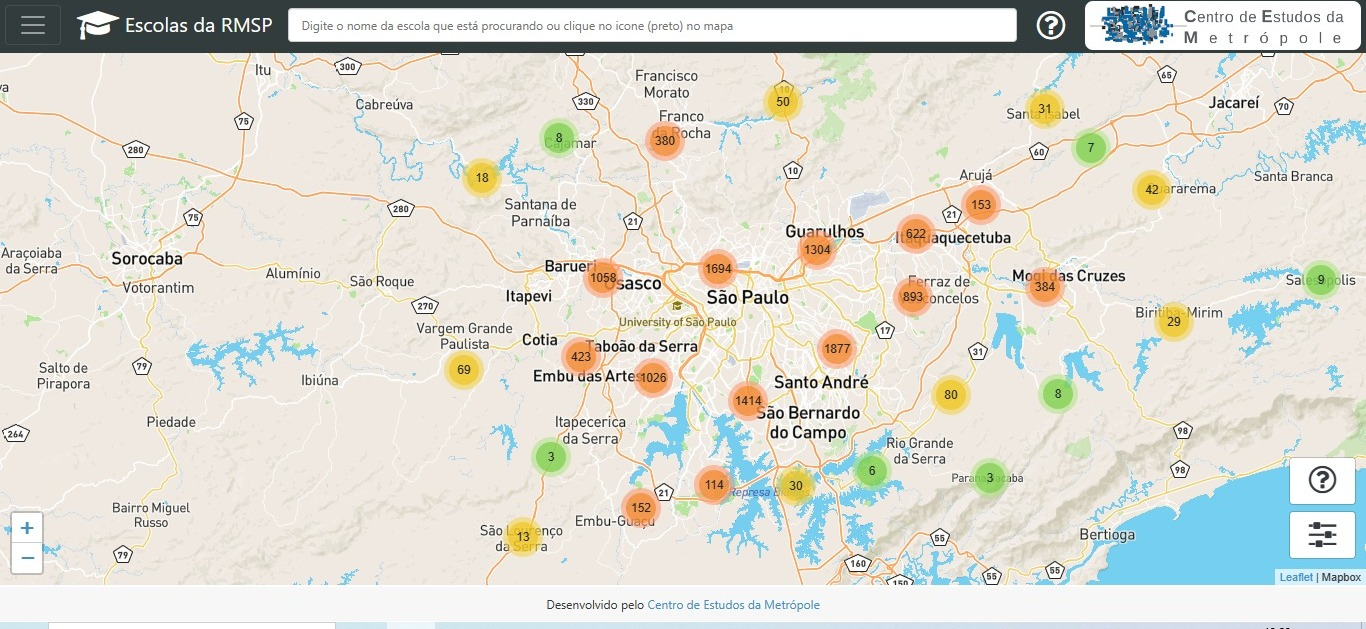
\includegraphics[width=\textwidth]{Figuras/siteCEM.jpeg}
    \caption{Mapa de clusters que mostra a quantidade de escolas em cada região. Ao aproximar o mapa, o usuário consegue ver a localização de cada uma das escolas presentes no banco de dados.}
    \label{fig:siteCEM}
\end{figure}

A segunda base coletada foi a base de dados da \href{https://prefeitura.pbh.gov.br/prodabel}{Prodabel}, empresa de informática e informação da prefeitura de Belo Horizonte. A base de dados foi descoberta por meio da referência 1. É uma base de dados mantida e atualizada mensalmente por 27 empresas públicas e privadas de Belo Horizonte. As empresas têm a responsabilidade de reportar qualquer inconsistência que encontrarem, bem como fornecer novos dados a medida que são adquiridos por ela. É uma base considerada confiável pois é constantemente atualizada e é utilizada por diversos serviços da prefeitura. Um exemplo de serviço que utiliza a base de dados é a distribuição dos alunos da rede pública por meio de georeferenciamento. A base conta com 740.000 endereços na data de coleta. A prefeitura também disponibiliza \href{https://bhmap.pbh.gov.br}{site com um mapa} para vizualização do endereços registrados. O endereço está posicionado em cima do edifício representado. Isso pode gerar erro de alguns metros devido a maioria da APIs colocar o endereço na frente do edifício representado. 

\begin{figure}
    \centering
    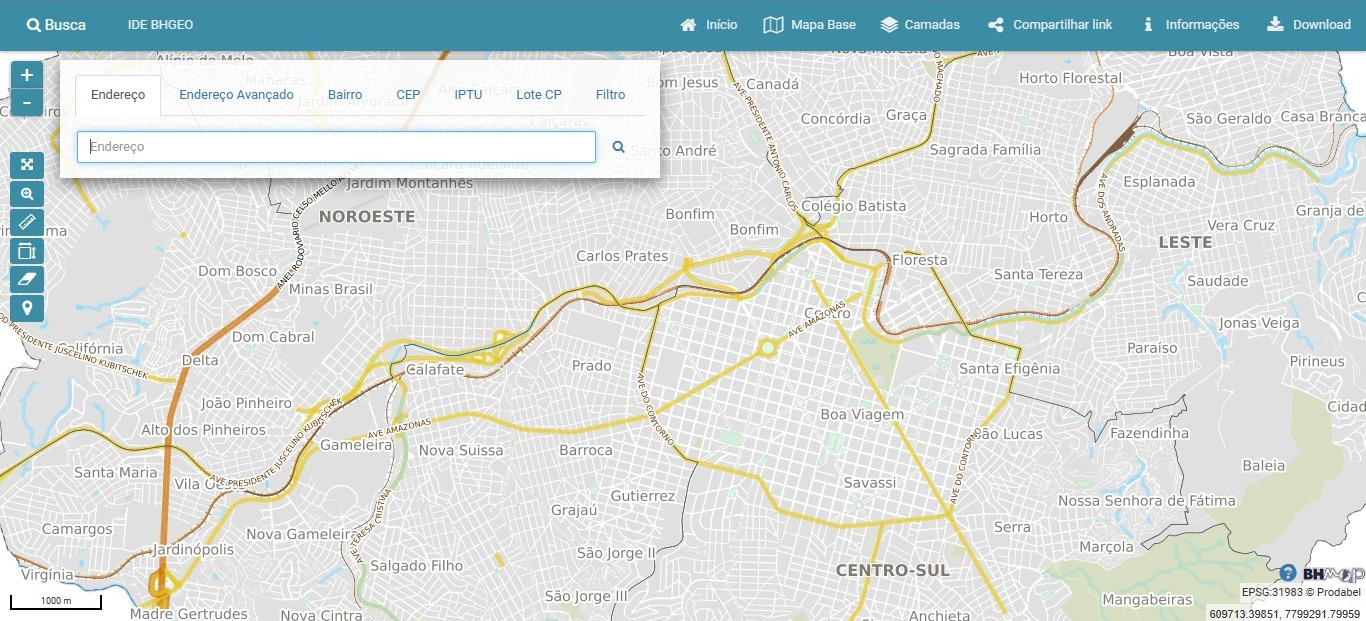
\includegraphics[width=\textwidth]{Figuras/siteProdabel.jpeg}
    \caption{Mapa que mostra a cidade de Belo Horizonte, desenvolvido pela Prodabel. Na barra de pesquisa, é possível pesquisar os endereços e marcá-los no mapa.}
    \label{fig:siteProdabel}
\end{figure}


\section{Processo de Geocodificação}

\begin{figure}
    \centering
    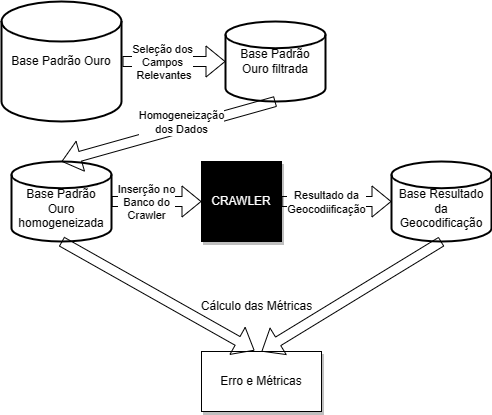
\includegraphics[width=\textwidth]{Figuras/diagrama monografia.drawio.png}
    \caption{Esquematização do processo de preparação e geocodificação dos dados}
    \label{fig:diagramaMono}
\end{figure}

A preparação de dados e geocodificação desempenham um papel crucial em muitos estudos e projetos que envolvem informações geográficas. Nesta pesquisa, esses processos desempenham um papel fundamental na obtenção de dados consistentes e na atribuição de coordenadas geográficas aos endereços.
A etapa de preparação de dados envolve a seleção dos campos relevantes da base de dados, como o nome da rua, número, bairro, CEP e cidade. Além disso, é realizada uma homogeneização dos dados, onde abreviações comumente utilizadas são substituídas por suas formas completas correspondentes. Essa etapa é essencial para garantir resultados mais precisos na geocodificação.
A geocodificação, por sua vez, consiste em atribuir coordenadas geográficas (latitude e longitude) a cada endereço presente na base de dados. Utilizando ferramentas adequadas, o processo de geocodificação é realizado, possibilitando a localização precisa de cada endereço no espaço geográfico.
Para realizar a geocodificação, os endereços previamente preparados são inseridos no banco de dados do Crawler, onde as ferramentas de geocodificação estão disponíveis. Essas ferramentas utilizam algoritmos e informações geográficas para identificar e atribuir as coordenadas geográficas correspondentes a cada endereço. É importante ressaltar que o processo de geocodificação é realizado pela equipe de Back-end do TerraLAB, portanto, vemos esse processo como uma caixa preta.
Uma vez concluída a geocodificação, os endereços geocodificados, juntamente com suas coordenadas geográficas, são armazenados no banco de dados. Esses dados geocodificados podem ser utilizados para análises espaciais, mapeamento e visualização de informações geográficas, contribuindo para a compreensão de padrões e tendências em determinada área de estudo.
Portanto, a preparação de dados e geocodificação são etapas essenciais para garantir a qualidade e a utilidade das informações geográficas utilizadas neste estudo. Esses processos permitem a obtenção de dados consistentes e georreferenciados, facilitando a análise e interpretação dos resultados obtidos

\section{Método de Avaliação}

\subsection{Erro, Acurácia e Discrepância}

A principal métrica utilizada para avaliar a qualidade da geocodificação é o erro do endereço. Esse erro é calculado como a distância entre o ponto de referência e o ponto geocodificado pela GeoAPI. Com base nesse erro, calcularemos medidas estatísticas, como a média, a mediana, o desvio padrão e a média aparada em 5\%, para analisar a precisão das GeoAPIs.

\begin{equation}
    e = D(p_{\text{Gold}}, p_{\text{Geo}})
    \end{equation}
    
    onde:
    \begin{itemize}
      \item $e$ é o erro da geocodificação,
      \item $D$ é uma função que calcula a distância em km,
      \item $p_{\text{Gold}}$ é o ponto da base Gold, e
      \item $p_{\text{Geo}}$ é o ponto resultante da geocodificação.
    \end{itemize}

    
Outra métrica utilizada é a taxa de resposta por API. Para alguns endereços da base de dados, as GeoAPIs podem retornar um erro, não fornecendo uma geocodificação válida. Nesse caso, nada é inserido no banco de dados. A taxa de resposta é calculada como a quantidade de endereços geocodificados dividida pela quantidade de endereços originais na base de dados. Esse valor, normalmente entre 0 e 1, é convertido em uma porcentagem para facilitar a compreensão dos resultados.
